\section{SAC头段变量}
\label{sec:sac-header-variables}

\subsection{基本变量}

\subsubsection{\texttt{nvhdr}*}
SAC头段版本号。\texttt{nvhdr}\footnote{星号表示该头段变量在SAC中必须
有定义值,下同。}是SAC中很重要但是不太常用的头段变量。目前版本号为6,
旧版本的SAC文件(\texttt{nvhdr<6})在读入时头段区会自动更新。

\subsubsection{\texttt{nzyear, nzjday, nzhour, nzmin, nzsec, nzmsec}}
分别表示``年''、``一年的第几天''\footnote{使用jday而不是``month+day''
可以少用一个头段变量。}\footnote{1月1日对应的 \texttt{nzjday} 是1而不是0。}、
``时''、``分''、``秒''、``毫秒''\footnote{\SI{1}{\s} = \SI{1000}{\ms}}。
这六个头段变量构成了SAC中唯一的绝对时刻,SAC中的其它时刻都被转换为相对
于该时刻的相对时间(单位为秒)。关于SAC中的绝对时间和相对时间的概念,
参考``\nameref{sec:sac-time}''一节。

根据这六个头段变量还可以推导出其它一些辅助型头段变量:
\begin{itemize}
\item \texttt{kzdate}:字符数字格式的参考日期,由 \texttt{nzyear} 和
    \texttt{nzjday} 导出
\item \texttt{kztime}:字符数字格式的参考时间,由 \texttt{nzhour}、
    \texttt{nzmin}、\texttt{nzsec}、\texttt{nzmsec} 导出
\end{itemize}

如下例所示:
\begin{SACCode}
SAC> fg seis
SAC> lh nzyear nzjday nzhour nzmin nzsec nzmsec

     nzyear = 1981
     nzjday = 88
     nzhour = 10
      nzmin = 38
      nzsec = 14
     nzmsec = 0
SAC> lh kzdate kztime

     kzdate = MAR 29 (088), 1981
     kztime = 10:38:14.000
\end{SACCode}

\subsubsection{\texttt{iztype}}
等效参考时刻。SAC的参考时刻是可以任意指定的,但一般选取某个特定的时刻
(比如文件起始时刻、发震时刻等等)作为参考时刻。其可以取如下枚举值
\footnote{枚举型在C源码中使用 \verb|#define| 宏来定义的,比如
\verb|#define IO 11|,所有可取的枚举值都以字母I开头。}:
\begin{itemize}
\item \texttt{IUNKN}:未知
\item \texttt{IB}:以文件开始时刻为参考时间
\item \texttt{IDAY}:以参考日期当天的午夜作为参考时间
\item \texttt{IO}:以事件发生时间为参考时间
\item \texttt{IA}:以初动到时为参考时间
\item \texttt{ITn}:以用户自定义的时间 \texttt{Tn} 为参考时间(n可取0--9)
\end{itemize}

若 \texttt{iztype=IO},则表示数据以发震时刻作为参考时刻,此时头段变量
\texttt{o} 的值应为0。

\subsubsection{\texttt{iftype}*}
SAC文件类型,其决定了头段区之后有几个子数据区。可以取如下枚举值:
\begin{itemize}
\item \texttt{ITIME}:时间序列文件(即Y数据,一般的地震波形数据)
\item \texttt{IRLIM}:频谱文件(实部-虚部格式)
\item \texttt{IAMPH}:频谱文件(振幅-相位格式)
\item \texttt{IXY}:一般的X-Y数据
\item \texttt{IXYZ}:一般的XYZ(3D)文件
\end{itemize}

\subsubsection{\texttt{idep}}
因变量(Y)类型,该头段变量可以不定义,其可以取如下枚举值:
\begin{itemize}
\item \texttt{IUNKN}:未知类型
\item \texttt{IDISP}:位移量,单位为 \si{\nm}
\item \texttt{IVEL}:速度量,单位为 \si{\nm\per\s}
\item \texttt{IVOLTS}:速度量,单位为 \si{\V}\footnote{不解}
\item \texttt{IACC}:加速度量:单位为 \si{\nm\per\square\s}
\end{itemize}

\subsection{数据相关变量}
\subsubsection{\texttt{npts}*}
数据点数,其值决定了在数据区有多少个数据点。

\subsubsection{\texttt{delta}*}
等间隔数据的数据点采样周期(标称值)。

\subsubsection{\texttt{odelta}}
采样周期的实际值,若实际值与标称值不同则有值,一般来说都是未定义的。

\subsubsection{\texttt{b*, e*}}
文件的起始时间和结束时间(相对于参考时刻的秒数)。

\subsubsection{\texttt{leven}*}
若数据为等间隔则为 \texttt{TRUE},否则为 \texttt{FALSE}。

\subsubsection{\texttt{depmin, depmax, depmen}}
因变量(Y)的最小值、最大值和均值。

在读入SAC文件以及对数据进行处理时,这三个头段变量的值会被自动计算并更新。
示例如下:
\begin{SACCode}
$ sac
SAC> fg seis
SAC> lh depmax
     depmax = 1.520640e+00      // 最大值
SAC> ch depmax 1000             // 强行修改数据最大值
                                // 这是错误的示范,不要这样做
SAC> lh depmax 1000             // 查看depmax,修改成功
     depmax = 1.000000e+03
SAC> w seis.SAC                 // 写到磁盘中
SAC> q
$ saclst depmax f seis.SAC      // 调用saclst查看磁盘文件中的depmax
seis.SAC         1000           // 可以看到磁盘中的文件depmax=1000
$ sac
SAC> r ./seis.SAC               // 读入SAC
SAC> lh depmax
     depmax = 1.520640e+00      // 此时depmax被自动计算并更新
\end{SACCode}

\subsubsection{\texttt{scale}}
因变量比例因子,即真实物理场被乘以该比例因子而得到现有数据。

假设真实物理场的Y值大概在$10^{-20}$量级,由于数据量级太小处理起来可能
不太方便。此时可以将数据乘以$10^{20}$变成合适的量级,并修改
\texttt{scale=}$10^{20}$,这样就可以知道自己对数据人为放大了多少倍。

101.5之前的版本中,在使用 \nameref{cmd:transfer} 命令去仪器响应时,
若 \texttt{scale} 的值有定义,则输出的数据会根据该值进行放大并修改
\texttt{scale}。在101.5及其之后的版本中,\texttt{scale} 被忽略。

\subsubsection{\texttt{xminimum, xmaximum, yminimum, ymaximum}}
仅用于3D(XYZ)文件中,记录X和Y的最小/大值。

\subsubsection{\texttt{nxsize, nysize}}
仅用于3D(XYZ)文件中,表示X和Y方向的数据点数。

\subsubsection{\texttt{iqual}\dag}
iqual\footnote{\dag 标识仅表示SAC程序内部未使用该头段变量,即变量有值
或者无值、有何值,对于程序的运行不会产生任何影响,但用户可以在自己的程序
中自由使用这些头段变量。下同。}标识数据质量,可取如下值:
\begin{itemize}
\item \texttt{IGOOD}:高质量数据
\item \texttt{IGLCH}:数据中有毛刺(glitches)
\item \texttt{IDROP}:数据有丢失(dropouts)
\item \texttt{ILOWSN}:低信噪比数据
\item \texttt{IOTHER}:其它
\end{itemize}

\subsubsection{\texttt{isynth}\dag}
合成数地震图标识。
\begin{itemize}
\item \texttt{IRLDTA}:真实数据
\end{itemize}

\subsection{事件相关变量}
\subsubsection{\texttt{kevnm}}
事件名,长度为16个字节。

\subsubsection{\texttt{evla, evlo, evel, evdp}}
分别代表事件的纬度(-90到90)、经度(-180到180)、高程(单位为 \si{\m},
未使用)和深度(单位为 \si{\km},以前为 \si{\m})。

\subsubsection{\texttt{ievreg}\dag}
事件地理区域\footnote{Flinn-Engdahl Regions:\url{http://en.wikipedia.org/wiki/Flinn-Engdahl_regions}}。

\subsubsection{\texttt{ievtyp}}
事件类型,这里仅列出部分常见的枚举值:
\begin{itemize}
\item \texttt{IUNKN}:未知事件
\item \texttt{INUCL}:核事件
\item \texttt{IEQ}:地震
\item \texttt{IOTHER}:其它
\end{itemize}

\subsubsection{\texttt{mag}}
事件震级。

\subsubsection{\texttt{imagsrc}}
震级信息来源,可以取如下枚举值:
\begin{itemize}
\item \texttt{INEIC}:\url{http://earthquake.usgs.gov/earthquakes/search/}
\item \texttt{IPDE}:\url{http://earthquake.usgs.gov/data/pde.php}
\item \texttt{IISC}:\url{http://www.isc.ac.uk/iscbulletin/search/catalogue/}
\item \texttt{IREB}:人工检查过的事件目录
\item \texttt{IUSGS}:\href{http://earthquake.usgs.gov}{USGS}
\item \texttt{IBRK}:\href{http://seismo.berkeley.edu/}{UC Berkeley}
\item \texttt{ICALTECH}:\href{http://www.seismolab.caltech.edu}{California Institute of Technology}
\item \texttt{ILLNL}:\href{https://www.llnl.gov/}{Lawrence Livermore National Laboratory}
\item \texttt{IEVLOC}:Event Location
\item \texttt{IJSOP}:Joint Seismic Observation Program
\item \texttt{IUSER}:The individual using SAC2000
\item \texttt{IUNKNOWN}:未知
\end{itemize}

\subsubsection{\texttt{imagtyp}}
震级类型,取如下枚举值:
\begin{itemize}
\item \texttt{IMB}:体波震级
\item \texttt{IMS}:面波震级
\item \texttt{IML}:区域震级
\item \texttt{IMW}:矩震级
\item \texttt{IMD}:持续时间震级
\item \texttt{IMX}:用户自定义震级
\end{itemize}

\subsubsection{\texttt{gcarc, dist, az, baz}}
\begin{itemize}
\item \texttt{gcarc}:全称Great Circle Arc,即震中到台站的大圆弧的长度,
    单位为度;
\item \texttt{dist}:震中到台站的距离,单位为 \si{\km};
\item \texttt{az}:方位角,震中到台站的连线与地理北向的夹角;
\item \texttt{baz}:反方位角,台站到震中的连线与地理北向的夹角。
\end{itemize}

\begin{figure}[H]
\centering
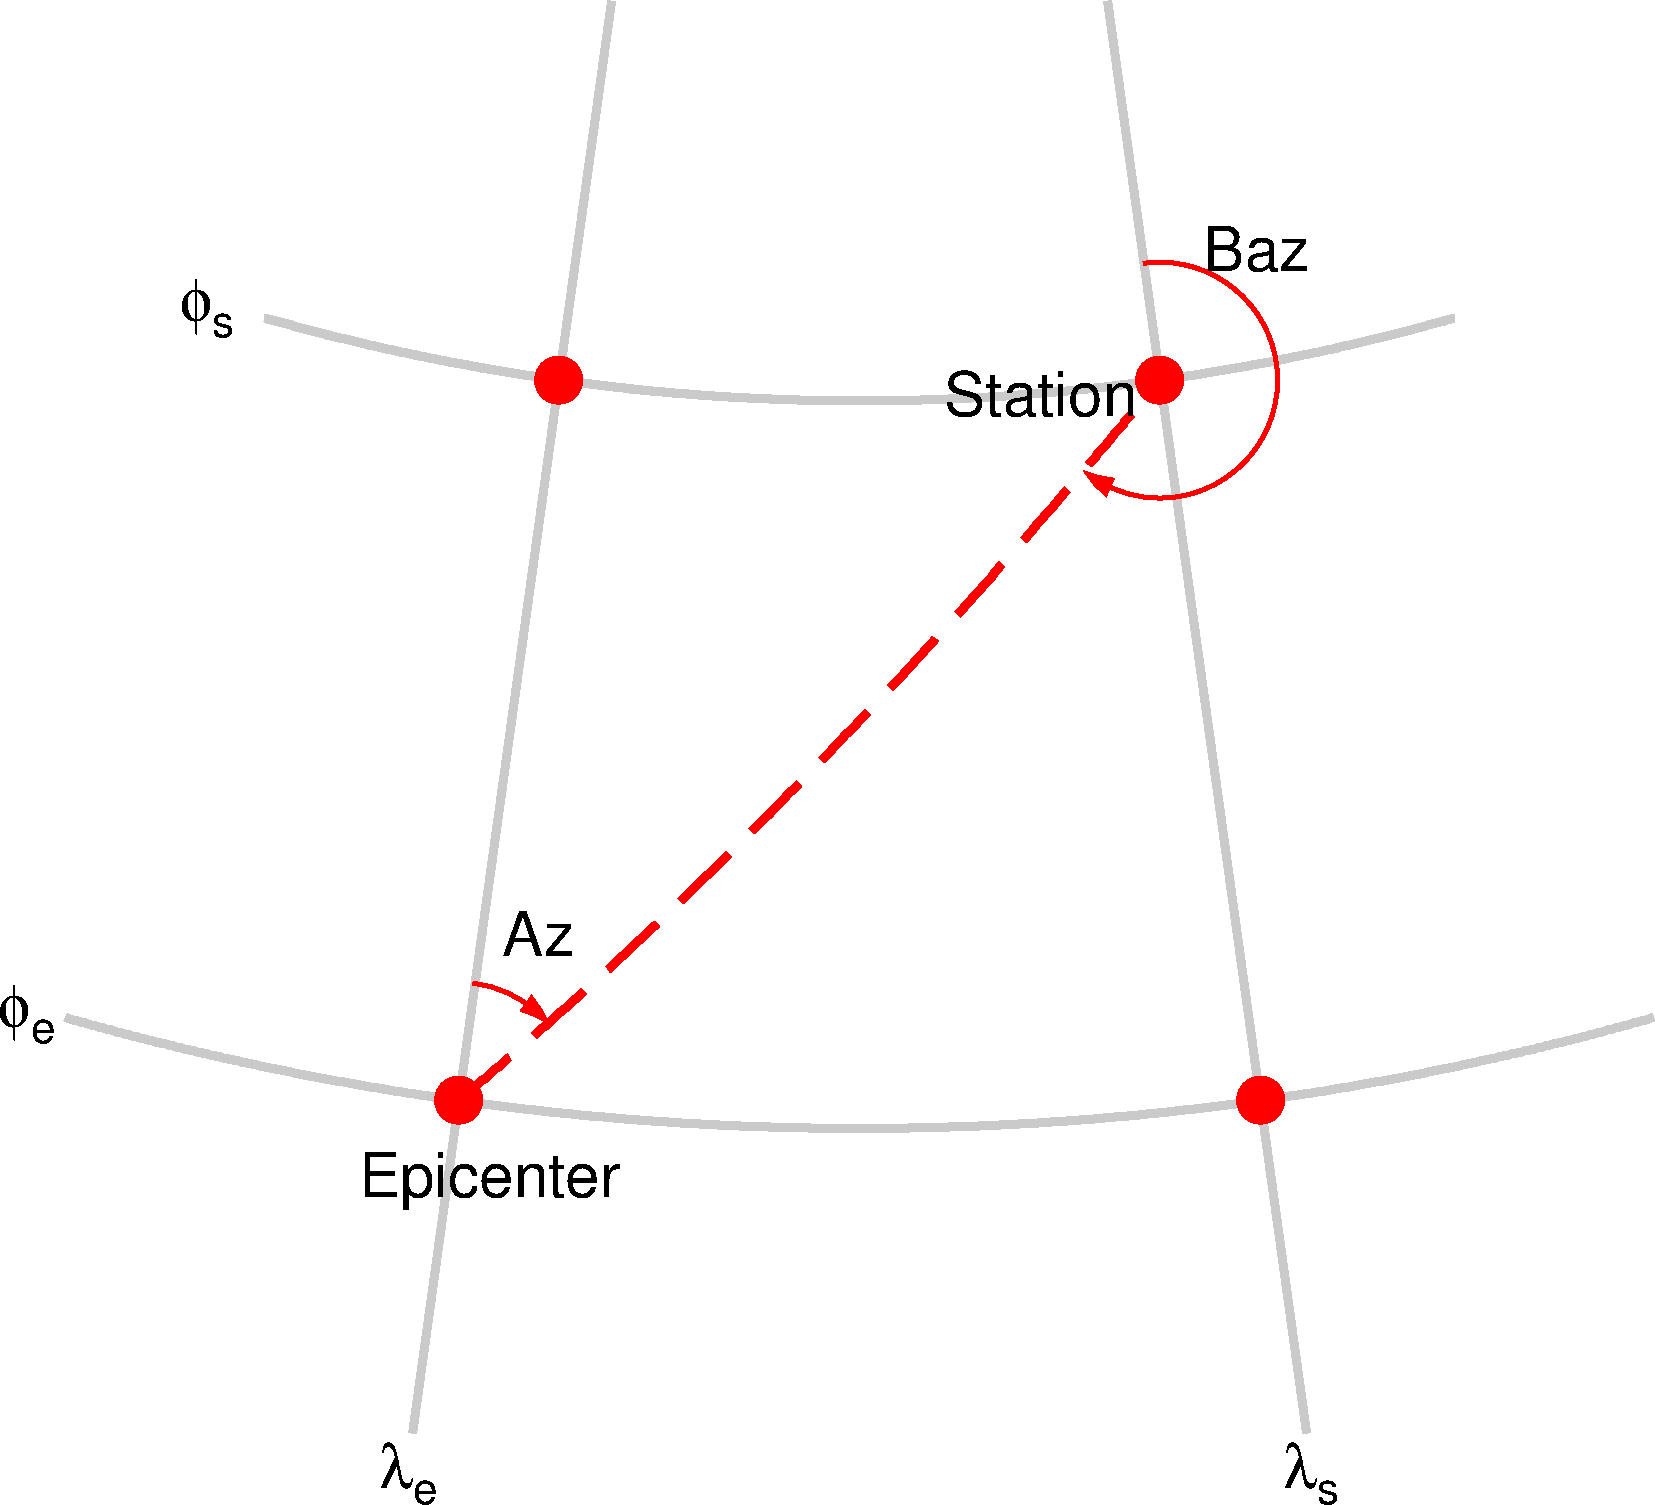
\includegraphics[width=8cm]{az-baz}
\caption[震中距、方位角、反方位角示意图]{震中距、方位角、反方位角示意图。}
\label{fig:gcarc-dist-az-baz}
\end{figure}

震中距、方位角和反方位角的计算涉及到球面三角的知识,具体公式及其推导
可以参考相关代码及书籍。此处列出部分仅供参考:
\begin{itemize}
\item \url{http://www.eas.slu.edu/People/RBHerrmann/Courses/EASA462/}
\item \url{http://www.seis.sc.edu/software/distaz/}
\item SAC源码 \texttt{src/ucf/distaz.c}
\item \href{http://www.eas.slu.edu/eqc/eqccps.html}{CPS330}源码 \texttt{VOLI/src/udelaz.c}
\end{itemize}

\subsubsection{\texttt{o, ko}}
\texttt{o} 为事件的发生时刻相对于参考时刻的秒数。\texttt{ko}是绘图时
时间变量 \texttt{o} 的标识符。

\subsubsection{\texttt{khole}}
若为核爆事件,则其为孔眼标识;若为其它事件,则为位置标识。

\subsubsection{\texttt{nevid, norid, nwfid}}
三者分别标识事件ID、起始时间ID和波形ID,仅用于CSS 3.0文件中。CSS 3.0
是SAC可以处理的一种数据格式,应该是当初SAC商业化的产物,目前仍保留
在SAC头段中。

\subsection{台站相关变量}
\subsubsection{\texttt{knetwk, kstnm}}
地震台网名和台站名。

\subsubsection{\texttt{istreg}\dag}
台站地理区域。

\subsubsection{\texttt{stla, stlo, stel, stdp}}
台站纬度(-90到90度)、经度(-180到180度)、高程(单位 \si{m},目前未使用)、
相对地表的深度(单位 \si{m},目前未使用)。

\subsubsection{\texttt{cmpaz, cmpinc, kcmpnm, kstcmp}}
一个台站至少需要三个正交的通道/分量才能完整地记录地面运动物理量。
\texttt{cmpaz} 和 \texttt{cmpinc} 指定了单个通道记录的方向矢量。

图 \ref{fig:cmpaz-cmpinc} 给出了SAC所使用的NEU坐标系,需要注意的是这是
一个左手坐标系。图中蓝色箭头为通道所记录的方向矢量,若地面运动与该方向
一致,则为正,否则为负。其中,头段变量 \texttt{cmpaz} 表征通道的方位角,
其定义为从N向开始顺时针旋转的角度,即图中的角度$\phi$;\texttt{cmpinc}
表征通道的入射角,定义为相对于U方向向下旋转的度数,即图中的角度$\theta$。

\begin{figure}[H]
\centering
\tdplotsetmaincoords{55}{50}
\pgfmathsetmacro{\rvec}{.8}
\pgfmathsetmacro{\thetavec}{30}
\pgfmathsetmacro{\phivec}{30}
\begin{tikzpicture}[scale=5,tdplot_main_coords]
\coordinate (O) at (0,0,0);
\draw[thick,->] (0,0,0) -- (1,0,0) node[anchor=south west]{$E$};
\draw[thick,->] (0,0,0) -- (0,1,0) node[anchor=south]{$N$};
\draw[thick,->] (0,0,0) -- (0,0,1) node[anchor=north east]{$U$};

\tdplotsetcoord{P}{\rvec}{\thetavec}{\phivec}
\draw[-stealth,color=blue] (O) -- (P);
\draw[dashed, color=red] (O) -- (Pxy);
\draw[dashed, color=red] (P) -- (Pxy);

\tdplotdrawarc{(O)}{0.2}{\phivec}{90}{anchor=west}{$\phi$}

\tdplotsetthetaplanecoords{\phivec}
\tdplotdrawarc[tdplot_rotated_coords]{(0,0,0)}{0.5}{0}%
{\thetavec}{anchor=south west}{$\theta$}
\end{tikzpicture}
\caption{\texttt{cmpaz} 和 \texttt{cpminc}示意图}
\label{fig:cmpaz-cmpinc}
\end{figure}

根据定义,地震仪标准通道的 \texttt{cmpinc} 和 \texttt{cmpaz} 值如下表:
\begin{table}[H]
\caption{标准地震通道的 \texttt{cmpaz} 和 \texttt{cpminc}}
\label{table:neu-cmpaz-cmpinc}
\centering
\begin{tabular}{ccc}
\toprule
方向    &   \texttt{cmpaz}   &   \texttt{cmpinc}  \\
\midrule
N       &   0       &   90          \\
E       &   90      &   90          \\
U       &   0       &   0           \\
\bottomrule
\end{tabular}
\end{table}

对于非标准方向的地震通道来说,很容易根据 \texttt{cmpinc} 和 \texttt{cmpaz}
的值,将其旋转到NEU坐标系或者RTZ坐标系,这些将在``\nameref{sec:traces-rotating}''
一节中说到。

\texttt{kcmpnm} 用于存储分量名称。SEED格式规定通道名的三个字符中的最后
一个代表通道的分量方位,比如通道名 \texttt{BHE} 表示该通道为东西向。
通常 \texttt{kcmpnm} 可以取为E、N、Z。由于很多台站的水平分量并不严格是
东西、南北方向,因而现在更倾向于用1和2代替N和E。

\texttt{kstcmp} 为辅助型变量,表示台站分量,由 \texttt{kstnm}、
\texttt{cmpaz}、\texttt{cmpinc} 推导得到。

\subsubsection{\texttt{lpspol}}
如图 \ref{fig:cmpaz-cmpinc} 所示,在左手坐标系下,若三通道都是正极性
则为真,否则为假。

\subsection{震相相关变量}
\subsubsection{\texttt{a, f, tn}}
\texttt{a} 和 \texttt{f} 用于存储事件的初动时刻和结束时刻相对于参考
时刻的秒数。

\texttt{Tn}(n=0--9)用于存储用户自定义的时刻相对于参考时刻的秒数,
常用于存储震相到时。

\subsubsection{\texttt{ka, kf, ktn}}
\texttt{a}、\texttt{f} 以及\texttt{Tn} 都有一个对应的以k开头的字符型
头段变量,称之为时间标识。时间标识用于说明对应的时间头段变量中所包含
时间的含义。

比如头段变量 \texttt{a} 中通常包含P波到时,则此时 \texttt{ka} 的值可以
设置为``P'';头段变量 \texttt{t1} 中包含了震相PcP的到时,则一般定义
\texttt{kt1} 为``PcP''。

在绘图时,若时间头段变量中有值,则默认会在该时刻处绘制一条垂线,若相应
的时间标记有定义,则将时间标记的值显示在垂线附近。

\subsubsection{\texttt{Xmarker}}
震相相关的变量对可以构成一个辅助型变量。\texttt{a} 和 \texttt{ka} 可以
构成\texttt{amarker},\texttt{f} 和 \texttt{kf} 可以构成 \texttt{fmarker},
\texttt{o} 和 \texttt{ko} 可以构成 \texttt{omarker},\texttt{tn} 和
\texttt{ktn} 可以构成 \texttt{tnmarker}(n=0--9)。

这些辅助型变量可以在 \nameref{cmd:listhdr} 中使用。

\subsection{仪器相关变量}
\subsubsection{\texttt{kinst}, \texttt{iinst}\dag, \texttt{respn}\dag}
\texttt{kinst} 为记录仪器的通用名称,\texttt{iinst} 为记录仪器的类型,
\texttt{respn} 为仪器相应参数。

\subsection{其它变量}
\subsubsection{\texttt{usern}}
\texttt{usern}(n=0--9)用于存储用户自定义的浮点型数值。

\subsubsection{\texttt{kusern}}
\texttt{kusern}(n=0--2)用于存储用户自定义的字符型值。

\subsubsection{\texttt{lovrok}}
若为 \texttt{TRUE},则磁盘里的原始数据可被覆盖;若为 \texttt{FALSE},
则原始数据不可被覆盖。主要用于保护原始数据,一般来说很少用到,若是出于
保护原始数据的目的,应优先考虑对原始数据做备份。

\subsubsection{\texttt{lcalda}}
全称为Calculate Distance and Azimuth。若为 \texttt{TRUE},则当事件和
台站的坐标被写入或被修改时,头段变量 \texttt{dist}、\texttt{gcarc}、
\texttt{az}、\texttt{baz} 将自动计算,否则不会被自动计算,SAC头段中
会存在信息的不兼容。

\subsubsection{\texttt{kdatrd}}
数据被读入计算机的日期(一般很少使用)。
